\documentclass[reprint,unsortedaddress,amsmath,amssymb,aps,prl,showkeys]{revtex4-2}
\usepackage{graphicx}% Include figure files
\usepackage{dcolumn}% Align table columns on decimal point
\usepackage{subfigure}
\usepackage{bookmark}
\usepackage{float}
\usepackage{url}
\usepackage{bm}% bold math
\usepackage{hyperref}% add hypertext capabilities
\usepackage[mathlines]{lineno}% Enable numbering of text and display math

\begin{document}

\title{Vicissitudes of Cities Driven by Re-distributive Growth}
\author{Gezhi Xiu, Jianying Wang, Lei Dong}
\author{Yu Liu}
\email{liuyu@urban.pku.edu.cn}
\affiliation{Institute of Remote Sensing and Geographic Information Systems (IRSGIS), Peking University}
\date{\today}

\begin{abstract}
	We propose a spatial growth model to address how cities emerge, grow, and especially, compete, over limited resource and space. The approach emphasizes on the evolutionary trajectory of cities, simultaneously determined by local (e.g., topography) and regional (e.g., industrial status) conditions, which can be attributed to the competition for redistributive resources in a given space. To model this spatial competition mechanism, our out-of-equilibrium growth model determines a fixed bound on global growth rates. We discuss two phases of urbanization predicted in our model: (a) free growth phase, and (b) resource constrained phase. Zipf's and Clark's laws in urban sciences are found in (a), indicating realistic urbanization process has not yet reached bottlenecks of resource; And when it reaches, (b) captures the inevitability of various urban diseases, e.g. urban shrinkage in developed cities and the spatial relocation of developments. Our approach sheds light on analyzing urbanization with early warnings of environmental capacity.
\end{abstract}
\maketitle

\textit{Introduction.} How do cities co-evolve over limited resource and space? To improve the conceptional understanding of urbanization and landscape evolution under complex circumstances, we need to set up some spatial growth models, i.e., a collection of models that derive macroscopic dynamical state given rules for every individuals. Such models are powerful tools to understand urban growth dynamics~\cite{PhysRevX.4.011008, Li2017Simple, makse1995modelling, rybski2013distance, nanda2017spatial}. Theoretically, these models fill the gap between macroscopic patterns, e.g. socio-economic scalars and material properties, and microscopic dynamics, e.g. individual level interaction patterns; Practically, they investigate how different growth factors contribute to city emergence, and how these dynamics lead to the observed scaling laws~\cite{bettencourt2007growth,court2013origins,batty2008size,batty2019urbanscalinglaw}, fractality~\cite{batty1994fractal,batty2007cities}, and city size distributions (i.e., Zipf's law)~\cite{zipf1949human}, giving quantitative references broadly through urban morphology and spatial structures for urban planers and policy makers~\cite{anas1998urban}. These existing works have built natural paths in deriving macroscopic dynamical state from microscopic growth rules. Most of these approaches are based on the assumptions of homogeneous growth in Euclidean geometry. However, recent discoveries of complex spatial phenomena associated with realistic urban systems are better described using fractal or discrete geometry\cite{makse1995modelling,louf2014congestion,PhysRevE.58.7054}, to better consist with growth dynamics in disordered contexts and media. From a individual perspective, existing models cannot incorporate spatially heterogeneous social group structures, e.g., ages\cite{PhysRevE.93.012112} and limited working chances. These call up a model with some simple mechanisms to include such information.

To capture the competitions, we develop a spatial growth model based on inconsistent space and memory-based growth dynamics. Here, new cities spontaneously emerge over free space, and a city is determined as the continuous surface that are developed by the same emergence. The spatial sprawl and the advance of urbanization are realized by the sequential settlement of new citizens. We claim that the location choice of the newly initiated citizens are adjacent to those limited total reserves of replacive \textit{active population}, keeping spatial preferential attachment and competition all at once. We show that beyond the desolated growth of each city, competitions introduced by spatial specialization and resource limit result in the vicissitudes of cities and urban shrinkage. Our model combines two themes for many disciplines, including probability theory and ecology: The spatial preferential attachment mechanism~\cite{Li2017Simple}, and the existence of environmental capacity under competition~\cite{gude2020bacterial,liu2019an}. 

% 刘老师意见:去掉On the first/second point On the first point, 
First off, the \textit{rich get richer} mechanism is well-observed in social systems, especially, human settlements are clustered hence cities~\cite{marsili1998interacting}. Literature has discussed how urban features emerge from preferential attachment via interaction density~\cite{ccolak2016understanding,louf2014congestion,fujita1976spatial}, e.g., multiplicative or correlated percolation~\cite{makse1995modelling,PhysRevE.58.7054,rybski2013distance}, spatial networks~\cite{marsili1998interacting,court2013origins,Li2017Simple}, and utility maximizing~\cite{PhysRevE.90.042815,axtell2001emergent}. Spatially, such mechanism leads to population clustering near every urban centers. Here, we take the spatial aspect from the idea of diffusion-limited aggregation~\cite{makse1995modelling, rybski2013distance, kleinberg2000navigation}, i.e., in each city, new comers would settle near those active citizens.

%On the second point, 
Secondly, cities are systems with environmental capacity, e.g., the governmental finance is supported by the city's parts of pillar industries, that excessive employees do not guarantee the proportional urban output. This is elaborated by finite technical demands and increasing infrastructural demand. In words, the marginal effect of urbanization leads to decreases in urban attractiveness~\cite{atkinson2012urban, girardin2009quantifying,gomez2018explaining,parris2003characterizing,batty2008size}. These are poorly reflected in the referred works, which are mostly base on certain equilibrium conditions or optimization aims~\cite{zipf1949human}. However, cities are inter-competitive and out-of-equilibrium to be consistent under circumstances towards sustainability\cite{fujita1976spatial,louf2014congestion,ccolak2016understanding}. Thus we include rules for spatial exclusiveness and bounded growth rate. Here, as also shown in non-spatial contexts~\cite{PhysRevE.55.R3817}, our restrictive settings intensify the inter-city competitions for active population\cite{batty2017urban}. We later prove that our space-relevant model extends the previous non-spatial predictions for city size distributions. These settings also result in realistic urban phenomena like ranking turnovers\cite{gabaix2004evolution}, and urban shrinkage\cite{haase2014conceptualizing}, that cannot be formulated by existing growth models.

\textit{Spatial Yule Model.} Our model tells how cities emerge, grow, and compete over space. Its dynamics are mainly determined through three quantitative and spatial rules: 1) \textit{Active citizen rule}. During urban growth process, we assume that only `active' citizens attract new comers to a nearby place in their city, $k$ and $N_i$ are the number of cities and active citizens in the $i$th city, respectively. 2) \textit{Memory kernel rule}. We take $\sum_{i} N_i \le N^*$ ($N^* \gg 1$) as the satiation condition, i.e., when the total population exceeds $N^*$, a new comer would deactivate a random dweller who is previously active. Equivalently, the kernel keeps up to $N^*$ active citizens adding up in the whole region. This rule also introduces the age structures in the population, since each kernel-labeled person is substituted with probability $1$ after a sufficiently long time. 3) \emph{Spatial growth rule}. We assume the studied area is an $L\times L$ 2-dimensional continuous space ($L\gg 1$) with grid of cells and periodic boundary conditions, %(IN THE BEGINNING, YOU SAID IT'S A continuous space?),
i.e., the locations of citizens are continuous, but the boundaries of cities are discrete on cells. A new city is seeded randomly over the region as a Poisson point process~\cite{miles1970homogeneous}, and survives if its cell is not taken; Every new citizen settles at a constant distance $r\le 1$ and a random angle $\theta$ from its introducer. Once a cell $c$ has held a citizen from the $i$th city, any citizens from another city $j$ ($j\ne i$) cannot introduce new comers on cell $c$. Thus cities are identified through citizens' ancestral introducer and their geographical occupation of blocks. The spatial growth rule is parallel Yule's settings on modeling the distribution of species per genus~\cite{yule1925ii}. So our model could be regarded as a spatial Yule model with constraints (SYM). A sketch for the SYM is shown in Fig~\ref{sketchpic}.

Based on these rules, we can define the model with a set of two-phase master equations. Specifically, we assume that the probability of a population increase in city $i$ within the time interval $(t,t+dt)$ is $\beta_2N_idt$, where $\beta_2$ is the introduction rate of every active citizen; We also assume that new cities constantly emerge with a small rate $\beta_1kdt$, proportional to the number of cities, where $\beta_1$ is the rate of new city generation. A city's generation is confirmed only if its location is at an empty cell. The master equation can be written as \begin{align}\frac{\partial}{\partial t}N_i(t) =  \delta_{N_i(t)}\cdot k\beta_1+ (1-\delta_{N_i(t)})\cdot N_i\beta_2, \end{align} for the free growth phase, where urbanization is weakly dependent with space and resource $N^*$;
%[WHAT'S THE DEFINITION OF FREE GROWTH?], 
and \begin{align}
	\frac{\partial}{dt} N_i(t) = \beta_2 N_i(t) -\delta_{\{\sum N_i = N^*\}}\cdot\notag \\ \left(\beta_1k(t) + (N^*-N_i(t))\beta_2 \right)
\end{align}
for the resource constraint phase, where the total resource $N^*$ are partitioned, and new dwellers get resource only through redistribution. 
%[WHAT'S THE DEFINITION OF RESOURCE CONSTRAINT PHASE?]. 

\begin{figure}
	\centering
	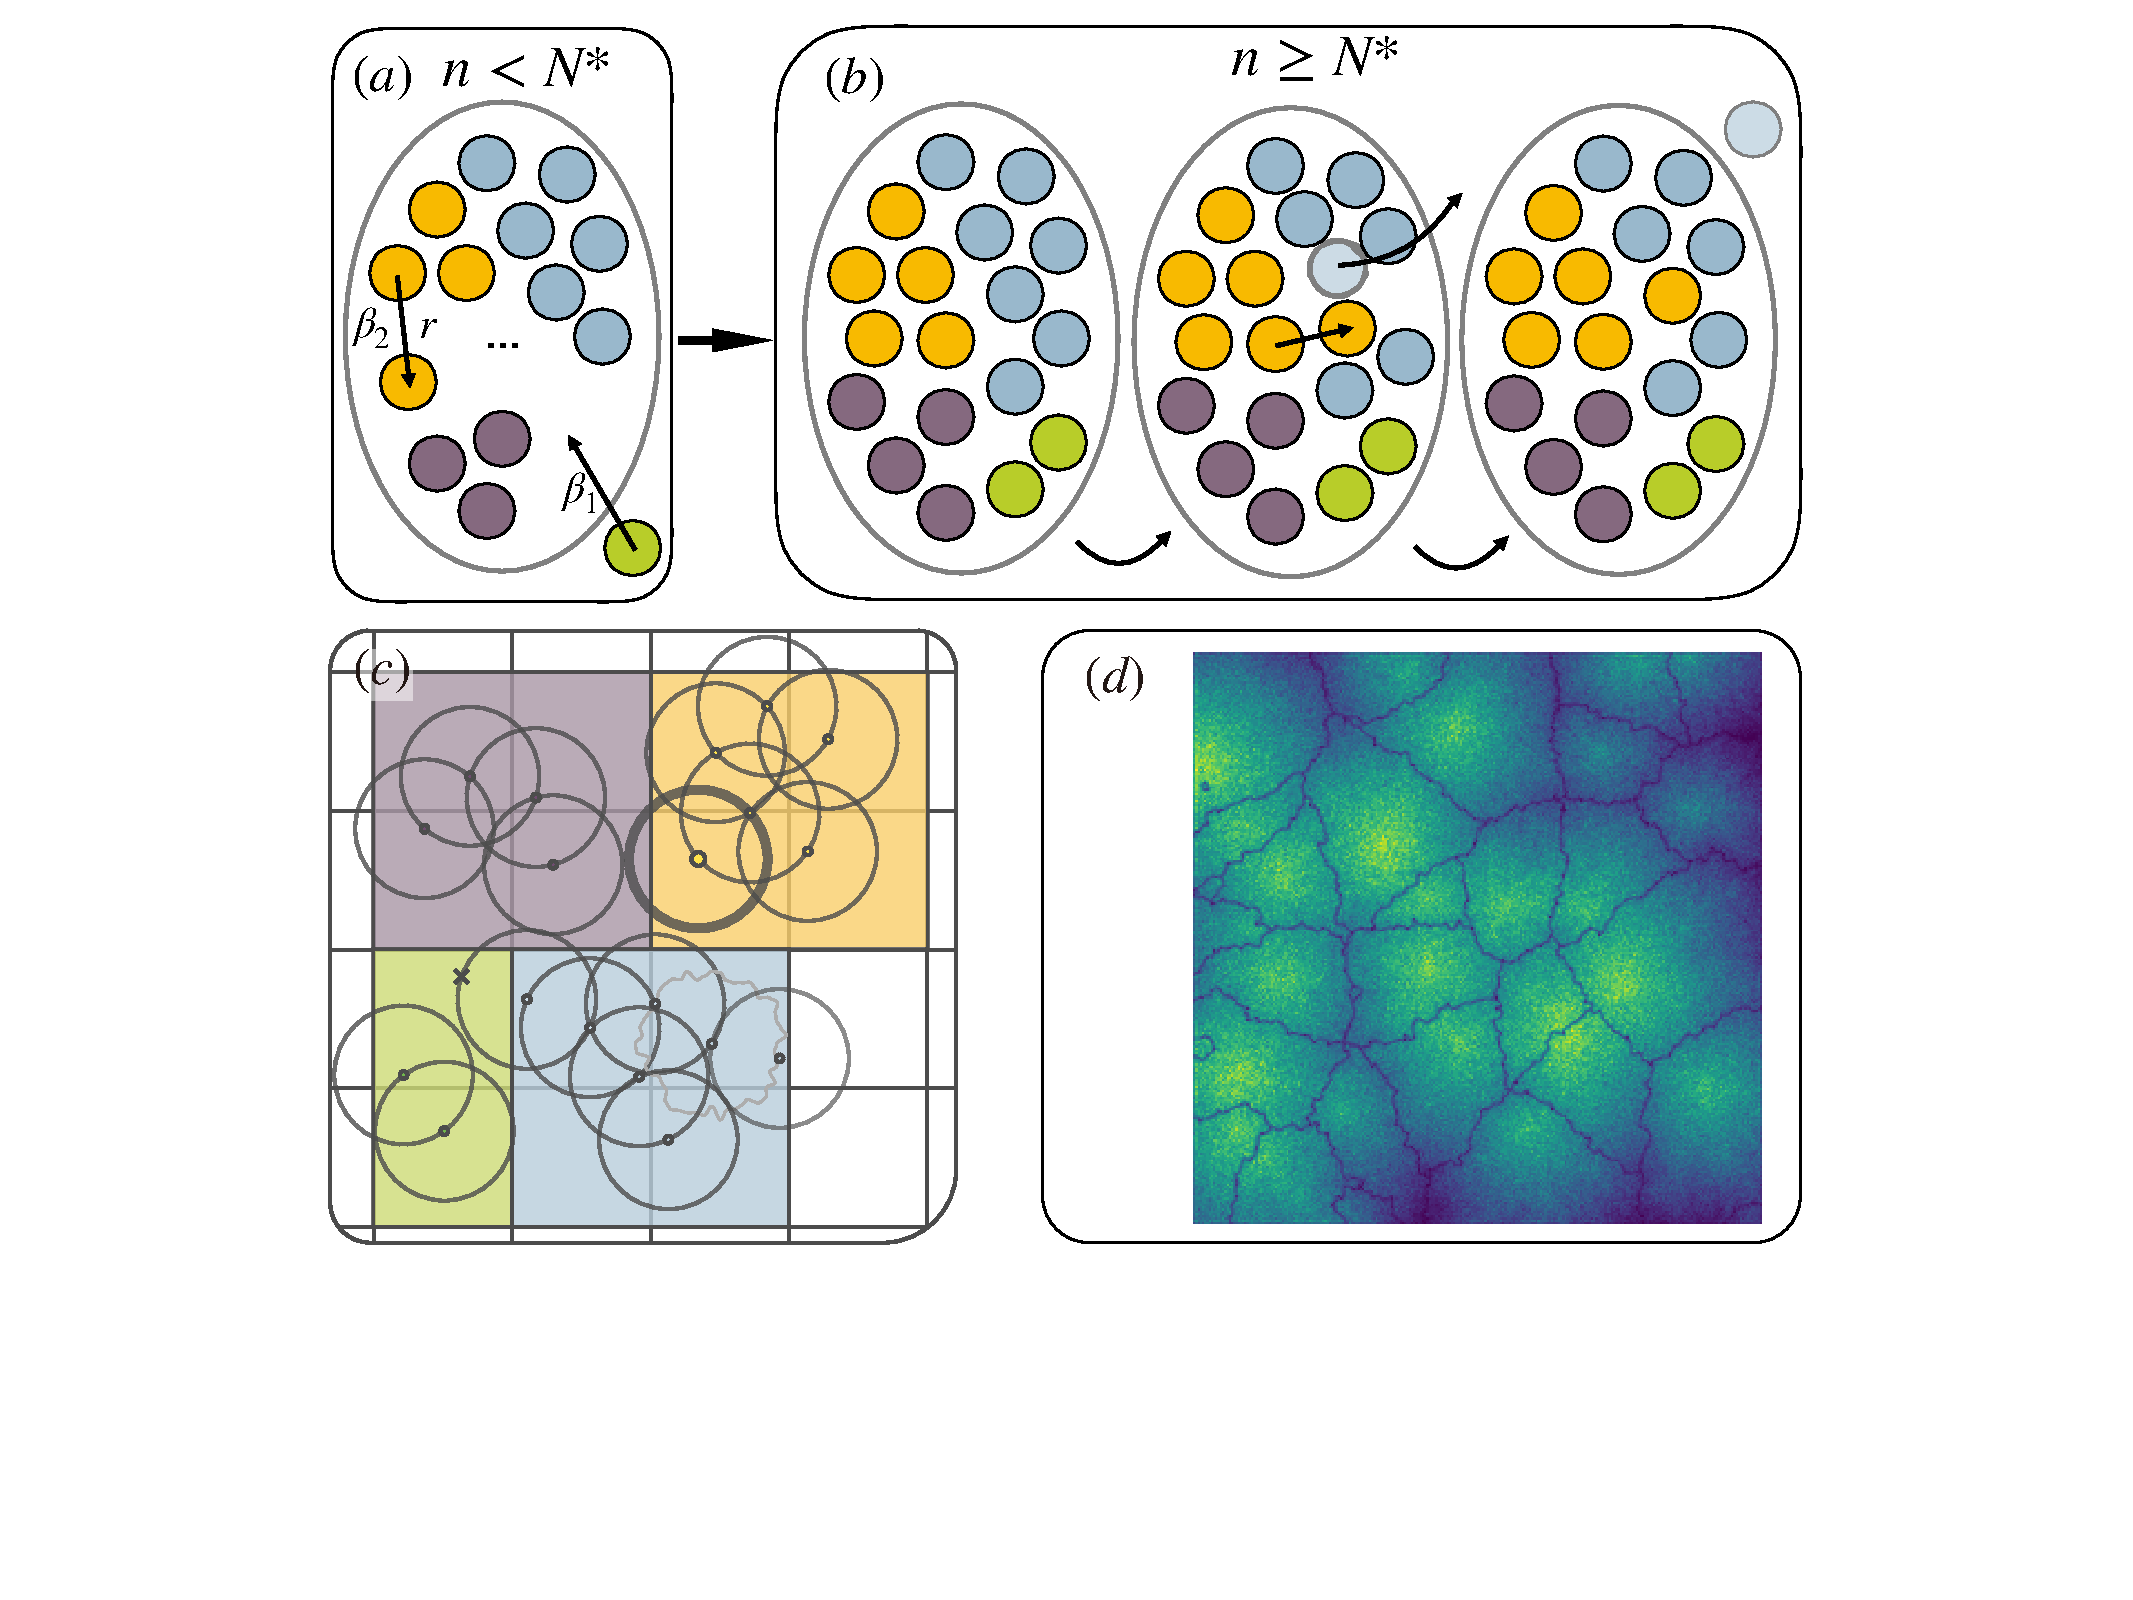
\includegraphics[width = 0.95\linewidth]{pics/sketchgood.pdf}
	\caption{\textbf{(a)} Status in the memory kernel at the free growth phase, i.e., the total population is less than $N^*$. Existing citizens introduce new dwellers at the rate $\beta_2$, while each existing city (noted by nodes in different colors) introduces new cities at the rate $\beta_1$. \textbf{(b)} When the memory kernel is fulfilled, every introduction of new city or citizen leads to an ejection of existing active citizen currently included in the memory kernel. \textbf{(c)} The spatial aspect is that, an offspring citizen's placement is at distance $r$ from the ancestral dweller. Also, when the kernel is filled, a new yellow node ejects an existed blue node, or equivalently deprive her ability to introduce. \textbf{(d)} A simulated result for $L$, $r$, $\beta$ equals to $256$, $0.5$, and $4$, respectively. We choose $\beta = 4$ to avoid confusion of too many cities. This is parallel to a quarter of $2L\times 2L$ simulation with $\beta = 1$.}
	\label{sketchpic}
\end{figure}

To summarize, the SYM can be regulated with three tunable parameters: the individual exploration distance $r$, the size of the memory kernel $N^*$, and the ratio $\beta:=\beta_2/\beta_1$. Though $\beta_1$ and $\beta_2$ have their actual meanings of generation speed, the model's dynamics and patterns are only determined by the relative growth rate $\beta$.

% 5. 模型需要哪些假设 6. 这些假设有什么理论和实证基础?
% [THE FOLLOWING PARA IS VERY CONFUSING. IF THIS IS ALSO RULES, YOU SHOULD PLACE THEM IN THE ABOVE PARA. IF THIS IS NOT, YOU SHOULD SPLIT THEM AND INSERT INTO THE PLACE THAT INTRODUCE PARAMETERS.] 
The model implies some simple assumptions. First, urban developments are density-driven. Literature has suggested that density-driven social ties and interactions comprise an important driver of the economies of scale~\cite{pan2013urban, girardin2009quantifying, batty1992form}. In the SYM, we further assume only the density of attractive population is corresponding to urban developments. Such active part can be recognized as the total employed or productive people. Second, to make an analytic framework, the growth dynamics are set to be homogeneous. The choices of place of new comers are random; The rate of introduction and emergence is the same for every active citizen and every city. This diffusive setting of sequential settlements is also realistic urban growth~\cite{RevModPhys.87.925}. 

In the numerical experiments, which is elaborated in \textit{SI}, the truly worth-tuning parameters are three, $\beta$, $r$, and $N^*$. $\beta$ contributes to the Zipf's coefficient and later defined turnover rate~\cite{rooney2006structural}; $r$ contributes to the fractality of urban areas and the time to fill the whole space; $N^*$ is the severeness of resource competition. 

% 7. 这个模型能推出哪些结论(1,2,3)。这些结论能如何被数据验证。
% \subsection{The free growth phase}

\textit{The free growth phase.} SYM predicts the existence of three phases of regional growth of cities, distinguished by whether resource and space have been fully occupied: freely growth phase, economic constraint phase, and spatial constraint phase. We focus on the first two phases, which correspond with regional resource. Spatial constraint phase's evolution implies a fully urbanized area, which is unlikely seen in reality, we discuss the situation only in \textit{SI}. In the freely growth phase, cities grow desolately, without being limited by resource and space. In this phase, SYM reformulates two important properties, stately (1) Zipf's law~\cite{gabaix1999zipf's} for rank size distribution of cities' population, and (2) Clark's law for exponential decay of urban density\cite{clark1951urban}. 

The populations of cities typically decay proportionally to the inverse of their ranks~\cite{gabaix1999zipf's}. This is referred as Zipf's law of cities' population sizes, i.e., the populations of cities distribute as a power of ranks, $f_r(r)\sim r^{-(1+\eta)}$. It is obvious that $N_i(t)$ has a geometric distribution~\cite{durrett1999essentials}, $P(N_i(t)=n)=e^{-\beta_1t}(1-\exp(- {\beta_1} t))^{n-1}$. Combining which with the assumption that the number of cities will grow exponentially at rate $\beta_1$, if we randomly pick an existing city, the waiting time since its first appearance is exponential with parameter $\beta_1$. Thus the distribution of population of a random city is 
\begin{align}
	f(n)=\frac{\Gamma(1+1/\beta)\Gamma(n)}{\beta\Gamma(n+1+1/\beta)}\approx Cn^{-1-1/\beta}, \ \text{as } n\to\infty,
\end{align}
where $\Gamma(\cdot)$ is Gamma function. This equation implies a Zipfian relationship with $n(\text{rank})\sim {rank}^{-\beta}$. Noticing that $\beta$ takes value from all positive real number in our model, we can derive arbitrary scaling behaviors by switching $\beta$. According to some studies~\cite{PhysRevLett.79.523}, the power law dependence of population frequency is $2.03\pm 0.05$ for the world, indicating that the average relative emerging rate of cities is around $1$. 

Varying $\beta$ also leads to the consideration of different sizes of study area. A small (large) $\beta$ interprets that the emergence of cities is fast (slow), corresponding to a large (smaller) study area. %[HOW ABOUT A LARGER BETA?] 
Thus varying $\beta$ is parallel to investigate the spatial density of cities in an urban system. Some urban systems tend to form new cities to have sufficient infrastructures and less diversity of urban output\cite{batty2008size} ($\beta > 1$) and some cities may go otherwise ($\beta< 1$). This value is actually a reflection of the intensity of regional population concentration in large cities. The experiments have confirmed our analytic results for free growth phase in SYM. %[I DON'T UNDERSTAND FROM `IT IS INTERESTING ... IN SYM. WHY THIS VALUE IS A REFECTION?] 
A simulated validation for this result can be reflected in Fig.~\ref{Fig2}. Notably, when $\beta$s are large ($>2$), the simulated Zipfian exponents are remarkably larger than their theoretical predictions. This is because the competition for space benefits small %[WHY LARGE SMALL CITIES?]
cities resulted from their higher density of edging cells, which is proved in \textit{SI}. For large $\beta$s, however, of the same rank, the probability of successful emergence of new city decreases due to relatively larger area of existing cities. This exasperates the concentration of active population in large cities.%% [UNCLEAR].
\begin{figure}[t]
	\centering
	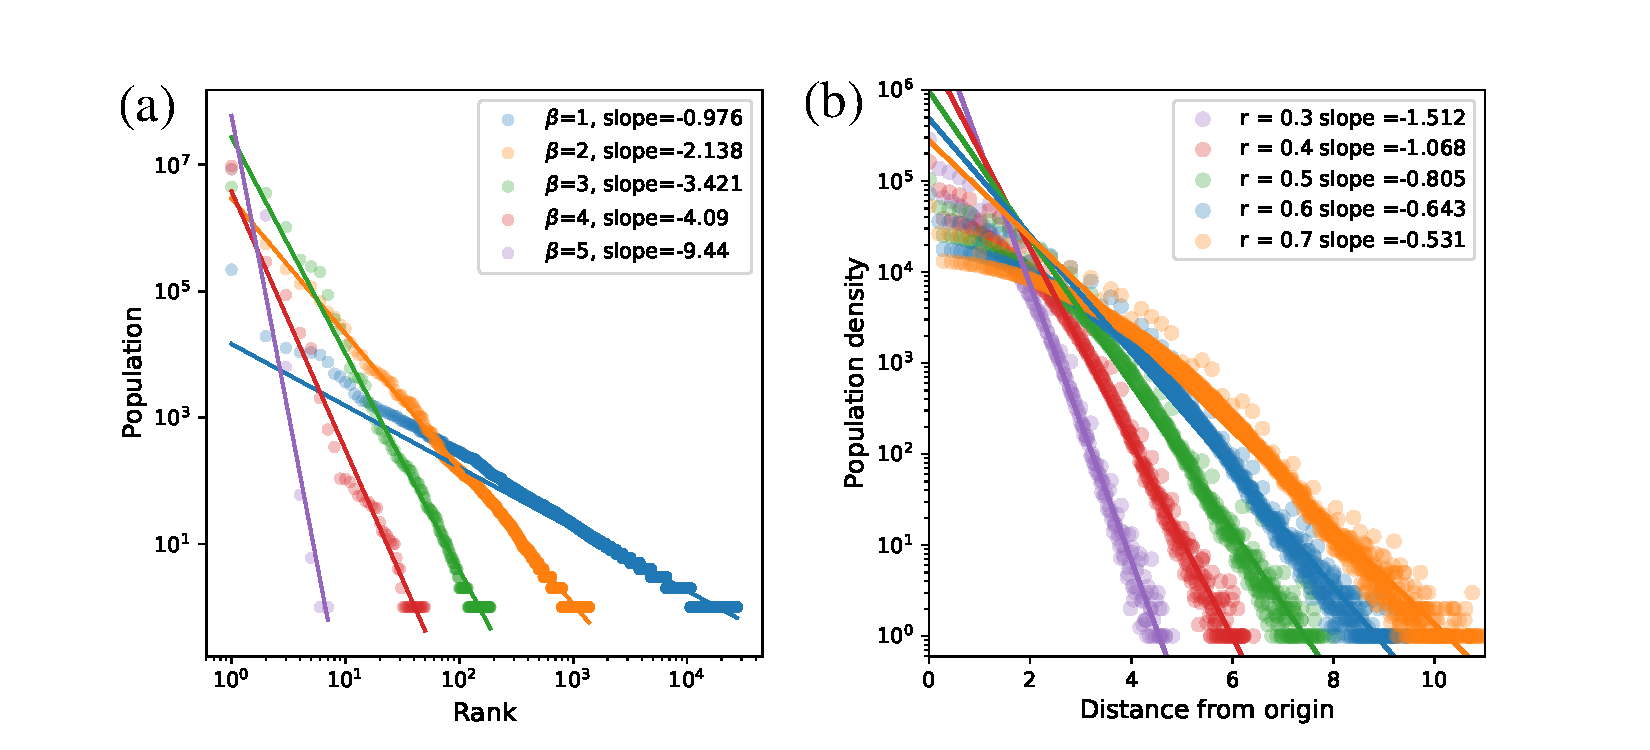
\includegraphics[width = .99\linewidth]{pics/Zipf_Clark.pdf}
	\caption{\textbf{(a)} The distribution of population among cities. In the simulation we take $N^* = 10^5$ and alternate $\beta$s. The realistic Zipf's coefficient is reproduced when $\beta\approx 1$. The theoretical predictions of the slopes are $-\beta$, and is well approximated when $\beta$s are small. Larger $\beta$ reduce the chance of latter city's emergence. Thus the spatial aspects of the SYM strengthen inequality. This result confirms that Zipf's law is valid for growing urban systems where all cities share the same rate to grow. From the other master equation we analyze that this observation vanishes if total growing force is finite. \textbf{(b)} The population distribution as a function of distance from a district's center for different step lengths $r$. The larger $r$ stands for the larger degree of flatten of a city. The vertical axis is logarithmic processed, which represents that the spatial population density decays exponentially for each $r$.}
	\label{Fig2}
\end{figure}

%% Clark
% [WHAT'S THE LOGIC SENTENCE FOR THE FOLLOWING PARA? I.E., WHAT'S THE CONNECTION BETWEEN THE FOLLOWING TO ABOVE-MENTIONED THINGS?]
SYM also revisits Clark's law in urban studies~\cite{clark1951urban}. In SYM, population density evolves as two-dimensional diffusion within a city\cite{doi:10.1137/0150099}, where we can focus the density's growth on each axis from the oldest citizens of a city. Let $
(d)$ denote the active population density of locations at the distance $d$ from a city center, and $t_n$ as the time for the $n$'th citizen to generate, we have 
\begin{align}
	\rho_{t_{n+1}}(d) = (\rho_{t_{n}}(d-r) + \rho_{t_{n}}(d+r) )/2.\label{loc_den}  
\end{align} By re-scaling time as $\tau_n = t_n\cdot (k\beta_1+N\beta_2)/T$, for a sufficient large $T$, this equation results in an exponential decay of density
\begin{align}
	\rho(d)\sim e^{-\alpha d}\label{clark_eq}.
\end{align} Details are presented in \textit{SI}. 

A direct implication of Clark's law is the competition strengths at urban edges, which also influence the local Zipfian exponents. From Clark's law, the population density is just a function of city's age and the distance from urban center. Specifically, the density at the edges is important since it determines the competition advantages for space. The population within an edging cell of city $j$ is estimated by $e^{(T-T_j)}\int_{d}^{d+1}\rho(r)dr/(2\pi d)$, where $T_j$ is the emerging time of city $j$. We also have the waiting time $T_{n+1}-T_{n}\sim 1/n$, and the total population approximation $e^{\beta_1+\beta_2}$, combining which we derive the density of edging cells if time and the urban radius are given. Since the attractiveness of large urban center is larger, the edging population of large cities is actually smaller than minor cities. We validate our prediction with simulations in Fig.\@\ref{Fig2}. %[DON'T FOLLOW UP THIS PARA, WHY IT HERE, WHY IT IMPORTANT?] %We give a detailed derivation in Appendix B\ref{edge_comp}.
In supplement, larger $r$ will weaken the above prediction, since the settlement are more even, thus larger proportion of citizens live at edges. In reality, the metropolis areas over the world have very different densities. In SYM, it corresponds to the sprawl of a city with given population. It can also be taken as the area proportion for a city in the studied region. On the other hand, it also controls the spatial limit of cities given competitionless population.

\textit{The economic constraint phase}. The multi-perspective coincidence between the exponents derived in our model and those in empirical evidences of population studies indicates that only two observation scales (the generation rates of city and citizen) lead to the behaviors of regional dynamics. This means that the actual urban growth has not yet reached the constrained cases. However, preventive measures are still necessary. Thus we bring a general constraining parameter $N^*$ to further discuss the second phase of SYM, the economy constraint phase, i.e., the total population reaches $N^*$. Such setting is the abstract of many real-life rules set by global organizations such as the allowance of carbon emissions or sustainable development projects. In each city, a proportion of population are active. Here, $\sum_{i=1} N_i(t) = N^*$ for $t$ that is sufficiently large. If in some period, the minor cities generate more offspring than major ones and the superiority of remaining population within the memory kernel changes, minor city will increase its ranking, as the growing rate for each city $i$ is actually $N_i\beta_2$. As for the dynamics within memory kernel, in each city, $N_i$ acts as a random walk with absorption wall $0$, since no offspring will be expected if no nodes are left in the kernel. This result also works for single cell case within a city. Denote the population with cell $j$ of city $i$ as $m_{ij}$. According to~\cite{durrett1999essentials}, we use a result for branching process that a cell loses its vitality if the population goes downhill under a threshold \begin{align}\rho_{threshold} = k/\beta.\end{align} This value shall be regarded as the sign for \emph{urban shrinkage}, for the edging cells have lower density according to equation~\ref{clark_eq} thus have an exponentially higher probability to be languished. In other words, urban shrinkage shall be reasoned by limited systematic resources. 

The kernel mechanism also plays a role at the cross-city scale: The preference of larger cities is easier to fail in a system with the memory kernel. The competition for active citizens in SYM receives more than pure birth settings because the sum of active population is given as $N^*$. In other words, SYM system doesn't consider natural growth. To test this interpretation, we analyze the turnover rate, defined as the average frequency of time steps in a realization that the second largest city surpasses the largest in active population. We conduct numerical experiments, and receive power law dependence of the frequency on simulating steps, shown in Fig.\@\ref{changerate}. Moreover, the switching is more likely to happen \textit{with} a memory kernel, i.e., turnover rate decay slower in probability if the system has constraints in resource. It is also a clear result since a growing society (a society without a memory kernel) suffer less from inter-specific competition.

\begin{figure}
	\centering
	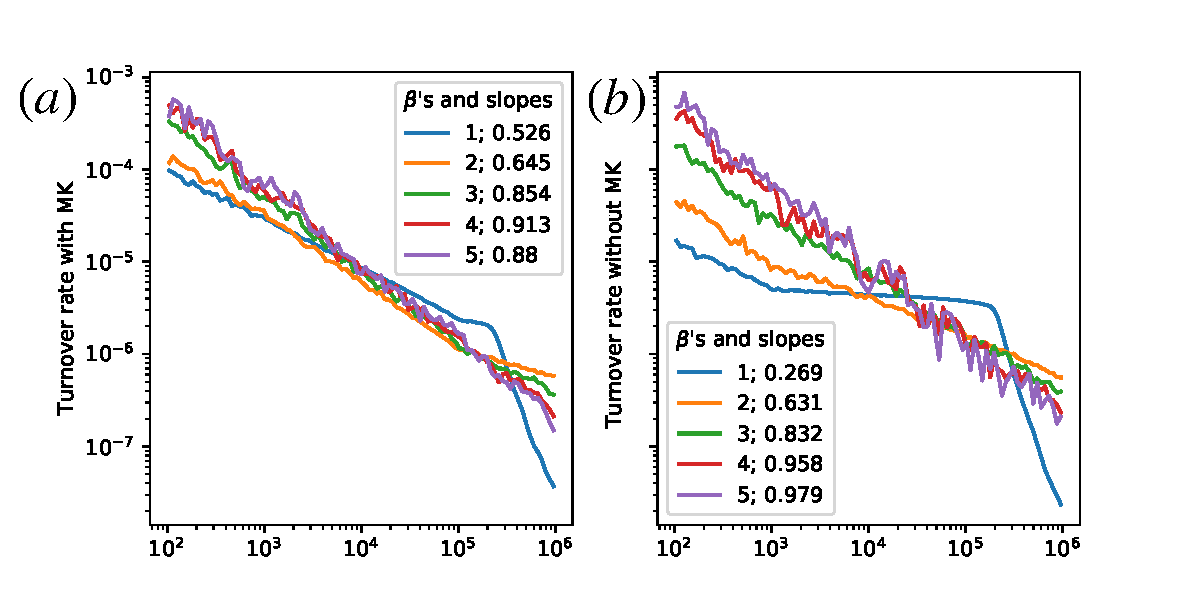
\includegraphics[width = 0.47\textwidth]{pics/turnoverrate.pdf}
	\caption{The change rate statistics with \textbf{(a)} and without \textbf{(b)} a memory kernel. The kernel keeps turning over more often. With same $\beta$'s, a kernel-based SYM's decay in turnover rate is smaller. These results validate our prediction that with finite resource, advantages are more likely to be kept.}
	\label{changerate}
\end{figure}

The last property of SYM is the fractality of urban envelop, stately, the length of urban edges vary with the used measurement. Inspired by multi-player interaction in fractal financial market\cite{PhysRevE.65.037106}, we interpret that fractal urban boundary is driven by the competition for land at cities' edges. In SYM, the uncertain competition for space lies in parameter $r$. A larger $r$ indicates larger randomness and brings an extra advantage for minor cities, resulting in a larger fractal dimension. We apply the box counting technique to calculate the fractal dimension of urban envelops, and receive an stable output of $d_f = 1.2\pm 0.05$ with $r = 0.5$, similar to empirical results\cite{batty1992form}. We also find larger $d_f$'s for greater $r$. These results validate our hypothesis that fractal edges coexist with spatial competition. Also, this result also confirms that SYM replicates an urban system.

% 总结我们这个模型的发现有哪些,为什么我们这个好。
\textit{Discussion.} In recent years, clearly we have witnessed the assumption of individual based models (IBMs) is deficient for multi-phased urban growth dynamics. The simplest approach is to modify the classical dynamical systems, adjusting the growth potentials via empirical derived geographical heterogeneity in the IBMs. This is not satisfactory since it confounds attempts to make extrapolations beyond the particular situations. An alternative, given the basis of economic complexity and the central place theory, is to derive causes of diversity, in which measures are developed abstracting the aggregated factors of production, and are predictive of future growth~\cite{Hidalgo10570}. It bridges a macroscopic dual to the IBMs. However, such an approach does not reach an end itself, for the economic complexity is even harder to monitor. 

In this \textit{Letter}, we have attempted to bridge the gap between IBMs and macroscopic descriptions for urban systems. The introduced memory kernel is a \emph{global} condition clarifying how the resources are shared by all cities: the governmental matching investment to allow introducing more new citizens. The recipient at different scales of this mechanism exhibits fruitful characteristics: Microscopically, it is a realization of system-conditioned spatial preferential attachment; In the intermediate level of cities, it introduces citizens' age structures and the accumulation of random shocks. The stationary age can be calculated as the average time for a new city to emerge is $(\beta_2 N^* + \beta_1 k)^{-1}$, which equals to the average losing age of the whole kernel. This result gives an instruction of the length of workable age in a given social urban system, elaborated in \textit{SI}. The global trends predicted in our model is more random than those non spatial and non-constraint models, allowing us to explained the vicissitude of cities, and the changes in spatial structures in the post-urbanization phase. Despite the model's simplicity, it is still capable of reformulating major aspects of empirical observations of urban population, including Zipfian ranking of cities by population size and Clark's law for urban population density. It also demonstrated the emergence of fractal urban edges. The generality of SYM can easily be embedded by spatial heterogeneous geographical circumstances, by adjusting the growing rate on each cell towards the product $m_{ij}\beta_2$, where $m_{ij}$ is the local characteristic.

% 不足
Although some results still need analytical proofs, this work is an essential step to strip out the power of urban dynamics. The model is non-commuting, but the community structure is naturally embedded. For further consideration, we can extend the model by adding links as the volume of exploration and preferential return between cities\cite{WANG2019121921}. The model can further be extended with multi-dimensional memory kernel, allowing one citizen to be introduced if different factors\cite{tokita2020social} (i.e., the existing citizens in different dimensions of kernel) agree to allow her in the system.



\bibliography{ref.bib}
% \begin{widetext}

\section*{Appendix}

The proofs presented in this section are all derived from the mean field approximations, which differ somehow from the simulated results. Their significance is the null results without random factors such as the spatial conditions.

\subsection{Zipf's law}

Zipf's law is the rank size distribution of cities. Denote by $q_m$ the number of cities having $m$ citizens, then $R(m) = \int_m^\infty q(m')dm'$ defines the rank. Empirically, $R(m)\sim m^{-1}$. The more populated a big city is, the more it is favored by up-comers. In study of city size distributions, SYM is a realization of \emph{the rich get richer} rule, for the city's growth rate increase proportionally with its present population. Thus, it is similar for cities size distributions to follow Zipf's law. 

The wait time for the $n$th citizen of a city to be born since the $n-1$th is $\frac{1}{\beta_2(n-1)}$. So inversely the expected population of a city at time $t$ is $e^{t\beta_2}$. We denote the sizes of cities at time $t$ as $n_i(t)$, for $i$ in $1,2,3,\dots$. Meanwhile, we denote the expected population of a city initiated $t$ ago as $Z(t)$. The transition probability of $P(Z_t = j)$ is $e^{-\beta_2 t}(1-e^{-\beta_2 t})^{j-1}$. Using Kolmogorov’s Forward Equation
\begin{align}p_t'(1,j) = -\beta_2 j p_t(1,j) + \beta_2 (j-1) p_t(1,j-1).\label{forward}\end{align}  When $j = 1$, we have \[p_t'(1,1) = -\beta_2 p_t(1,1), \] which leads to $p_t=e^{-\beta_2}$. When $j>1$, we differentiate $P(Z_t = j)$ to have 
\begin{align}
	\frac{dP(Z_t = j)}{dt} &= -\beta_2e^{-\beta_2 t} (1-e^{-\beta_2 t})^{j-1} + e^{-\beta_2 t}(j-1)(1-e^{-\beta_2 t})^{j-2}\beta_2 e^{-\beta_2 t}\notag\\
	&= -\beta_2 e^{-\beta_2 t}(1-e^{-\beta_2 t})^{j-1} + e^{-\beta_2 t}(j-1)(1-e^{-\beta_2 t})^{j-2} [-(1-e^{-\beta_2 t})\beta_2+\beta_2]\notag\\
	&= -\beta_2 e^{-\beta_2 t}(1-e^{-\beta_2 t})^{j-1} -\beta_2 e^{-\beta_2 t}(j-1)(1-e^{-\beta_2 t})^{j-1} +\beta_2e^{-\beta_2 t}(j-1)(1-e^{-\beta_2 t})^{j-2}\notag\\
	&= -\beta_2 j e^{-\beta_2 t}(1-e^{-\beta_2 t})^{j-1} +\beta_2e^{-\beta_2 t}(j-1)(1-e^{-\beta_2 t})^{j-2}
\end{align}
which copes with equation \ref{forward}. Thus we complete the proof of the probability distribution of a city's population. The probability distribution of the region's population is easy to find according to the given result. The probability distribution of registering $j$ people in $i$ cities at time $t$, is \[ P_t(i,j) = \left(\begin{array}{c}{j-1} \\ {i-1}\end{array}\right)\left(e^{-\beta t}\right)^{i}\left(1-e^{-\beta t}\right)^{j-i}. \] 

Moreover, tuning the mechanism from pure birth to birth-death process, we receive a different scaling factor.

\subsection{Clark's law}

In this part, we use the mean-field approach to derive the spatial distribution of population within a species. This quantity can be interpreted as the spatial distribution mode of a species. The good thing about the mean-field approach is that we can use the potential concept to derive some conclusions. Here, we regard the growing mechanism as a multi-dimensional binary tree. On each dimension, the tree's $i$th layer has $i$ potential nodes. The probability on the $i$th node's generation is is the average of the two nearest nodes' potential generation probability. Basing on the homogeneity of the choice of $\theta$, the derivation along different axis is the same. Within each city, the spatial distribution of people are captured by the introducing mechanism, $(r,\theta)$. Clark's law\cite{clark1951urban} and some variations for multi-centered models\cite{griffith1981modelling} are empirical clues that correspond to such spatial distributions. Here we reformulate the Clark's law under spatial Yule principles. Since the isotropic setting, the derivation is only needed in one dimension added on a Doppler effect. When spatial constraints are neglected, the expected density distribution along an axis from the origin has an exponential form,$\rho (R)\sim e^{-\alpha R}$. We start the discussion as a node being placed on a broad area. Regardless of adding nodes on else axis, the second is placed at $r$ right-side of the first with a probability of $1/2$. Along this axis, the $n$th node is placed at $k$ from the right end with $C_n^k/2^n$. Using the Stirling formula, it approximately equals to \begin{align}
    & \frac{n^{n+1/2}}{\sqrt{2\pi}k^{k+1/2}(n-k)^{n-k+1/2}}\notag                         \\
=    & \frac{n-k}{k+1}\frac{(1+\frac{1}{n-1-k})^{-k-1/2}}{(1+\frac{1}{k})^{n-k-1/2}}\notag \\
=    & \frac{n-k}{k+1}\frac{(1+\frac{1}{n-1-k})^{n-k-1/2}}{(1+\frac{1}{k})^{k+1/2}}\notag  \\
\sim & e^{-k},
\end{align}
which turns out to be a exponential distribution. We can interpret it as the local properties of spatial Yule model is a discrete version of a maximum entropy system, since the Clark's law can also be derived by maximum entropy principle\cite{merity2009accurate}. Recalling the simple mobility assumption as random walk in random direction, we show that individual-level diffusion process can be approximated by the sum of really simple moves.This is a non-trivial result since this is not derived by mean field approach but by random walk assumption of human mobility. To make it precise, at the early stage of the process, a new community can land near the centre of an existing one. In reality, two communities that are too adjacent are sometimes illustrated as two \emph{districts} in the same city. In our model, a set of communities that destruct others' roundness functions the same with districts within one city. 

By alternating the distributions of step length, we can reproduce other forms of people density distributions. A more skewed distribution of $r$ brings a Levy-like mobility pattern. In particular, a power law mobility distribution brings a Zipf's density distribution $\rho '(R)\sim R^{-\gamma}$\cite{PhysRevX.4.011008}, where $\gamma$ is the scaling factor.  In the following part, we focus on global characteristics to derive the area and population distributions among communities.

\subsection{Competition at the edges}
We consider the individual level expansion at urban edges. We denote that the distance between the first and the furthest node of a city as $O$ and $F$, respectively, and the moment that $F$ lands its first offspring as $t+\tau$, where $t$ is the moment that $F$ is landed. We investigate the radius of the city, which is defined by the distance between $O$ and $F$. The radius of a city at time $t$, $R_t$, changes to $R_{t+\tau}$ when the offspring is given birth. The expectation of $R_{t+\tau}$ goes as 
\begin{align}
	E R_{t+\tau} &= \int_0^{\frac{\pi}{2}} \sqrt{(R_t+r\cos\theta)^2+(r\sin\theta)^2} d\theta \notag \\
	&= \sqrt{2 R_t r} \int_{0}^{\frac{\pi}{2}} \sqrt{\frac{R_{t}}{2 r}+\frac{r}{2 R_{t}}+\cos \theta} d \theta \notag\\
	&= 2(R_t+r) \mathbb{E}\left(\pi/4| \frac{4R_t r}{(R_t+r)^2}\right)
\end{align}where $\mathbb{E}$ is the elliptic function. We find that it decreases as $r$ increases. So that the smaller cities have more active edging cells.

\subsection{Average Age within the Memory Kernel}

We consider the active population over the whole region as working population. The generation speed of population is $N^*\beta_2 + k\beta_1$. Thus the population is refreshing, leading to a constant expected age of \[N^*/\beta'\] for $\beta' := (N^*\beta_2 + k\beta_1)/N^*+k$. This leads to a practical implication that the working age allowed in cities shall be related with the sum of working offer from central government of a region. For instance, in the United States, the regressive value of $\beta$ is around $0.04$. We assume that the working years of a person is 40 years, the expected $N^*$ for the United States is 1,600 units, i.e., 4 millions distributive working opportunities in all cities.


\section{Details on the simulations}

The simulation results presented here are obtained in the following way. Instead of conducting the designed protocol, we do it in an equivalent way by stretching timeline to events labeled in integer. At each time step, we first decide if we add a new city, with probability $p(S)$, or a new meta-population to the existing city, with probability $1-p(S)$. The probability $p(S)$ is determined by the total regional population and number of cities, $\frac{k\beta_1}{k\beta_1+N\beta_2}$. If a city is to be built, the place of it is randomly chosen at an empty spot. By empty we mean the cell of the spot contains no existing node. If it is a new node to be generated, we first determine its ancestor node, and land it at $(r,\theta)$ of the ancestor node, where $r$ is constant default as $0.5$ and $\theta$ is a realization of a uniform distributed random variable $\mathcal{U}[0,2\pi]$. The new generations of nodes are accompanied with a record in the memory kernel (MK).


\section{Illustrations for the economic constrained phase}

\subsection{Turnover rate} 

Regional development is complex and is affected by different determinants in different time. For example, in Hebei province of China, the largest city Shijiazhuang started to develop fast since it is the crossroad of railways. We interpret this as the redistribution of social resource. There have been plenty of literature\cite{bowles2019neolithic} that illustrate the interplay between social development and injustice. Regional development is complex and is affected by different determinants in different time. For example, in Hebei province of China, the largest city Shijiazhuang started to develop fast since it is the crossroad of railways. Jilin City in Jilin province used to be the capital of Jilin province until Changchun, from 1954, replaced its status. Obviously, these are redistributions of social resource. In many literature, social injustice is strengthened by the technical revolutions. Stately, agricultural society is more likely to store fortune overtime than nomadic society\cite{doi:10.1086/701789}. The Gini coefficients in ancient society is also increasing as the productivity grows\cite{kohler2017greater}. We read this as inequality of human society is born with the desire of better life. 

But what is more interesting is that, when doesn't the rich get richer? In this Letter we give a possible explanation that the \emph{memory} of human society is the force of future endeavour. A city's future ability to develop is based on the active population brought by the existing active people. The limited resource is dynamically divided by increasing number of cities, so that there is, though small, but still some odd of overturn. In the following text, we first derive an approximated solution of this problem. We denote the coins share in the $k$th largest city as $n_k$, and investigate the probability that the second largest city becoming the largest, $P_{\text{overturn}}$. In $m$ successive additions of meta-population from the moment $t_l$, the chance for $n_2(t_l+m)\ge n_1(t_l+m)$ is equivalent to the case that the city $2$ is picked $n_1(t_l)-n_2(t_l)$ times more than city $1$. The probability of $n_1(t_l)-n_2(t_l)$ picks of city $2$ in a row is $\frac{n_1!}{n_2!}/N^{n_1-n_2}$. Adding another step brings an probability of $n_1/N$ for $n_1$ to increase to $n_1+1$. So the process ends at $n_1(t_l)-n_2(t_l)+1$ steps is the former probability times $(n_1+1)/N$ and plus a expected latent step length. 

\subsection{Urban shrinkage}

The urban development is a sequel of the spatial distribution of existing resource. Thus the preferential attachment is not only performed among people, but also on urban land-use. The concentration of urban resource result in urban shrinkage, indicating that the popular definition of resource distribution, say Gross Democratic Product (GDP), may not be the best indicator of regional fortune, since it is not a perfect indication of a place's future. Urban shrinking is widely discussed in recent years. It is always referred with demographic changes such as decreasing fertility, aging, and out-migration\cite{haase2008urban}. In the comprehension of urban input-output framework, the governmental investment cannot follow up with the spatial growth of population. So the further investment can only go to \emph{active} area where recent comers to the cities are mostly found. 

We conduct a cell-wise analysis. The speed of a cell's losing active population equals to the speed of others' adding, $[(N^*-n)\beta_2 +k \beta_1]\cdot n/N^*$; The speed of its own adding is $n\beta_2$. Thus the equilibrium condition is \[ [(N^*-n)\beta_2+k\beta_1]\cdot \frac{n}{N^*} = \beta_2N^*. \] The equilibrium $n_eq = k/\beta$. This means that whether a spot in city will be prosperous  has nothing to do with the regional resource $N^*$, but it is related to the strong force of emergence of cities.
\end{widetext}
\end{document}